\documentclass[12pt,a4paper,spanish,openany
]{book}
\usepackage[spanish]{babel}
\usepackage{amsmath}
\usepackage{graphicx}             
\usepackage{amsfonts}
\usepackage{amssymb}
\usepackage{graphics}
\usepackage{indentfirst}
\usepackage{enumerate}
\usepackage{fancyhdr}
\usepackage{fancybox}
\usepackage{lastpage}
\usepackage{color}
\usepackage{amsbsy}
\usepackage{amsthm}
\usepackage{listings}
\usepackage{titlesec}
\usepackage{titletoc}
\usepackage{subfig}
\renewcommand{\baselinestretch}{1}
\clubpenalty=10000
\widowpenalty=10000
\usepackage{makeidx}%glosario de términos
\usepackage[all]{xy}
\numberwithin{equation}{section}
\theoremstyle{definition}
\newtheorem{defi}{Definición}[chapter]

\theoremstyle{definition}
\newtheorem{propo}{Proposición}[section]

\theoremstyle{definition}
\newtheorem{coro}{Corolario}[section]

\theoremstyle{definition}
\newtheorem{teorema}{Teorema}[section]

\theoremstyle{definition}
\newtheorem{ejercicio}{Ejercicio}[section]

\theoremstyle{remark}
\newtheorem{ejemplo}{Ejemplo}[section]

\usepackage{srcltx}%permite la busqueda inversa, si no viene por defecto en la version de LaTeX usada.

% lo siguiente solo usarlo cuando compilo directamente en pdflatex
% si lo uso compilando en latex el {\'\i}ndice no lo hace bien
\usepackage{hyperref}

\hypersetup{colorlinks=true, linkcolor=black, urlcolor=black, citecolor=black}
\hypersetup{bookmarksopen=false, bookmarksnumbered=true} \hypersetup{pdfstartview=FitH}

\makeindex

\usepackage{pdfpages}
\setlength{\parskip}{5pt plus 2pt minus 1pt}
%%%%%%%%%%%%%%%%
%%% MACROS
%%%%%%%%%%%%%%%%

\newcommand{\cplx}[1]{{{\mathcal #1}^{\scriptscriptstyle\bullet}}}

\newcommand{\dmc}[1]{{D}^-(#1)}
\newcommand{\dbc}[1]{{D}^b(#1)}

\newcommand{\fmf}[3]{{\Phi^{#1}_{{\scriptscriptstyle #2\!\rightarrow\! #3}}}}
\newcommand{\lotimes}{{\,\stackrel{\mathbf L}{\otimes}\,}}

\newcommand{\cO}{{\mathcal O}}
\newcommand{\cP}{{\mathcal P}}
\newcommand{\cE}{{\mathcal E}}
\newcommand{\cG}{{\mathcal G}}
\newcommand{\calL}{{\mathcal L}}
\newcommand{\cI}{{\mathcal I}}
\newcommand{\cF}{{\mathcal F}}
\newcommand{\cQ}{{\mathcal Q}}
\newcommand{\cM}{{\mathcal M}}

\newcommand{\f}{\mathfrak{f}}

\newcommand{\iso}{{\,\stackrel {\textstyle\sim}{\to}\,}}
\newcommand{\what}[1]{{\widehat #1}}

\newcommand{\rk}{\operatorname{rk}}
\newcommand{\ch}{\operatorname{ch}}
\newcommand{\Td}{\operatorname{Td}}
\title{Temario 3º de la ESO}
\author{Pedro Ángel Fraile Manzano}
\date{2023}
\usepackage[left=2cm,right=2cm,top=2cm,bottom=2cm]{geometry}
\begin{document}
\maketitle
\tableofcontents
\chapter{Operaciones sobre $\mathbb{Q}$}

\noindent El conjunto de los números racionales $\mathbb{Q}$ es el conjunto que se pueden dar  como una pareja de números enteros. 

\begin{defi}
Llamaremos numerador al número entero que está arriba en la fracción.
\begin{equation}
\dfrac{a}{b}\text{ El término a}
\end{equation}
\end{defi}

\begin{defi}
Llamaremos denominador al número entero que está abajo en la fracción.
\begin{equation}
\dfrac{a}{b}\text{ El término b}
\end{equation}
\end{defi}
\section{Suma y resta de Fracciones}
\noindent Cuando tienes un par de fracciones sólo se pueden sumar si tienen el mismo denominador. 

\noindent Para sumar dos fracciones \textbf{con el mismo denominador}, basta con mantener el denominador y se suman los denominadores:
\begin{equation}
\dfrac{a}{b}+\dfrac{c}{b}=\dfrac{a+c}{b}
\end{equation}

\noindent En el caso de que no tengan el mismo denominador hay que dar la siguiente definición:
\begin{defi}
Dos fracciones $\frac{a}{b}, \frac{c}{d}$ son equivalentes si se cumple que :
\begin{equation}
 a\cdot d=b\cdot c
 \end{equation} 
\end{defi}
\begin{ejemplo}
Las fracciones $\frac{3}{5}, \frac{6}{10}, \frac{12}{20}$ son equivalentes
\end{ejemplo}

\noindent Hay que definir el concepto de \emph{fracción irreducible}

\begin{defi}
Una fracción es irreducible si el máximo común divisor del numerador y el denominador es 1. 
\end{defi}

\begin{ejemplo}
La fracción $\frac{14}{16}$ es reducible, ya que el máximo común divisor es $2$, dividiendo entre $2$ tanto denominador como el numerador obtendremos la fracción irreducible $\frac{7}{8}$
\end{ejemplo}

\noindent Un método para obtener fracciones equivalentes es multiplicar denominador y numerador por el mismo número. 

\begin{ejemplo}
Las fracciones $\frac{3}{5}=\frac{3\cdot 4}{5\cdot 4} =\frac{12}{20}$ son equivalentes
\end{ejemplo}

\noindent Para sumar dos fracciones con denominadores distintos se sigue el siguiente procedimiento:
\begin{enumerate}
\item Se calcula el mínimo común múltiplo de los denominadores. 
\item Se divide el mínimo común múltiplo por cada uno de los denominadores.
\item Se multiplica el numerador y el denominador por el resultado de la división. 
\end{enumerate}

\noindent De esta manera, se obtienen dos fracciones que son equivalentes a las anteriores pero con el mismo denominador. 

\begin{center}
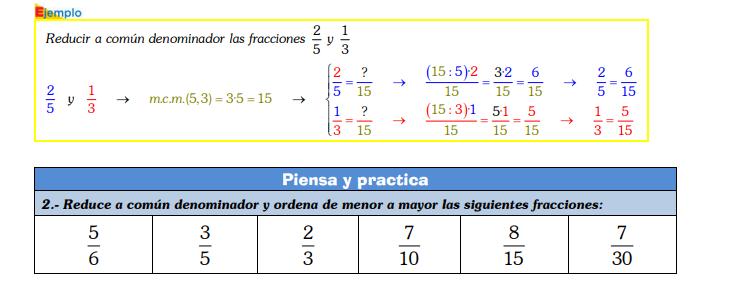
\includegraphics[scale=0.75]{C:/Users/Pedro/Documents/apuntes-particulares/3º de la ESO/Imágenes/Tema1-ejercicio1.png}
\end{center}
\includepdf[fitpaper=true,pages={7}]{C:/Users/Pedro/Documents/apuntes-particulares/3º de la ESO/Ejercicios/Ud01_Racionales.pdf}

\section{Producto y la división de Fracciones}

\noindent Para realizar el producto de fracciones, basta con multiplicar los numeradores y los denominadores entre si.

\noindent Para la división se sigue el siguiente esquema:
\begin{center}
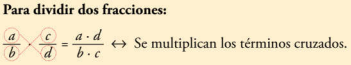
\includegraphics[scale=0.75]{C:/Users/Pedro/Documents/apuntes-particulares/3º de la ESO/Imágenes/Division_fracc.png}
\end{center}

\begin{defi}
Llamaremos \emph{fracción inversa} de una fracción a la que cambia los términos, es decir la que cambia denominador y numerador
\begin{equation}
\dfrac{a}{b} \Rightarrow \dfrac{b}{a}
\end{equation}
\noindent Otra propiedad es que si las multiplicas entre sí es $\dfrac{a}{b}\cdot\dfrac{b}{a}=\dfrac{ab}{ba}=1$
\end{defi}

\begin{center}
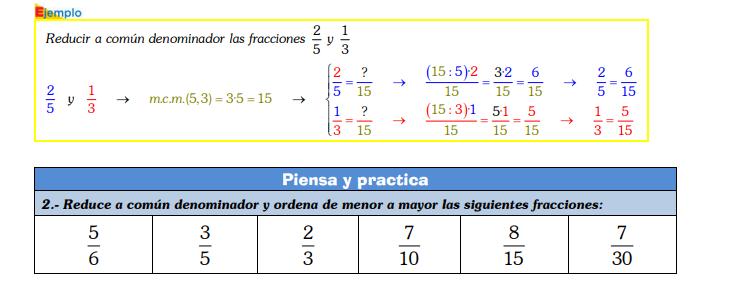
\includegraphics[scale=0.75]{C:/Users/Pedro/Documents/apuntes-particulares/3º de la ESO/Imágenes/Tema1-ejercicio1.png}
\end{center}

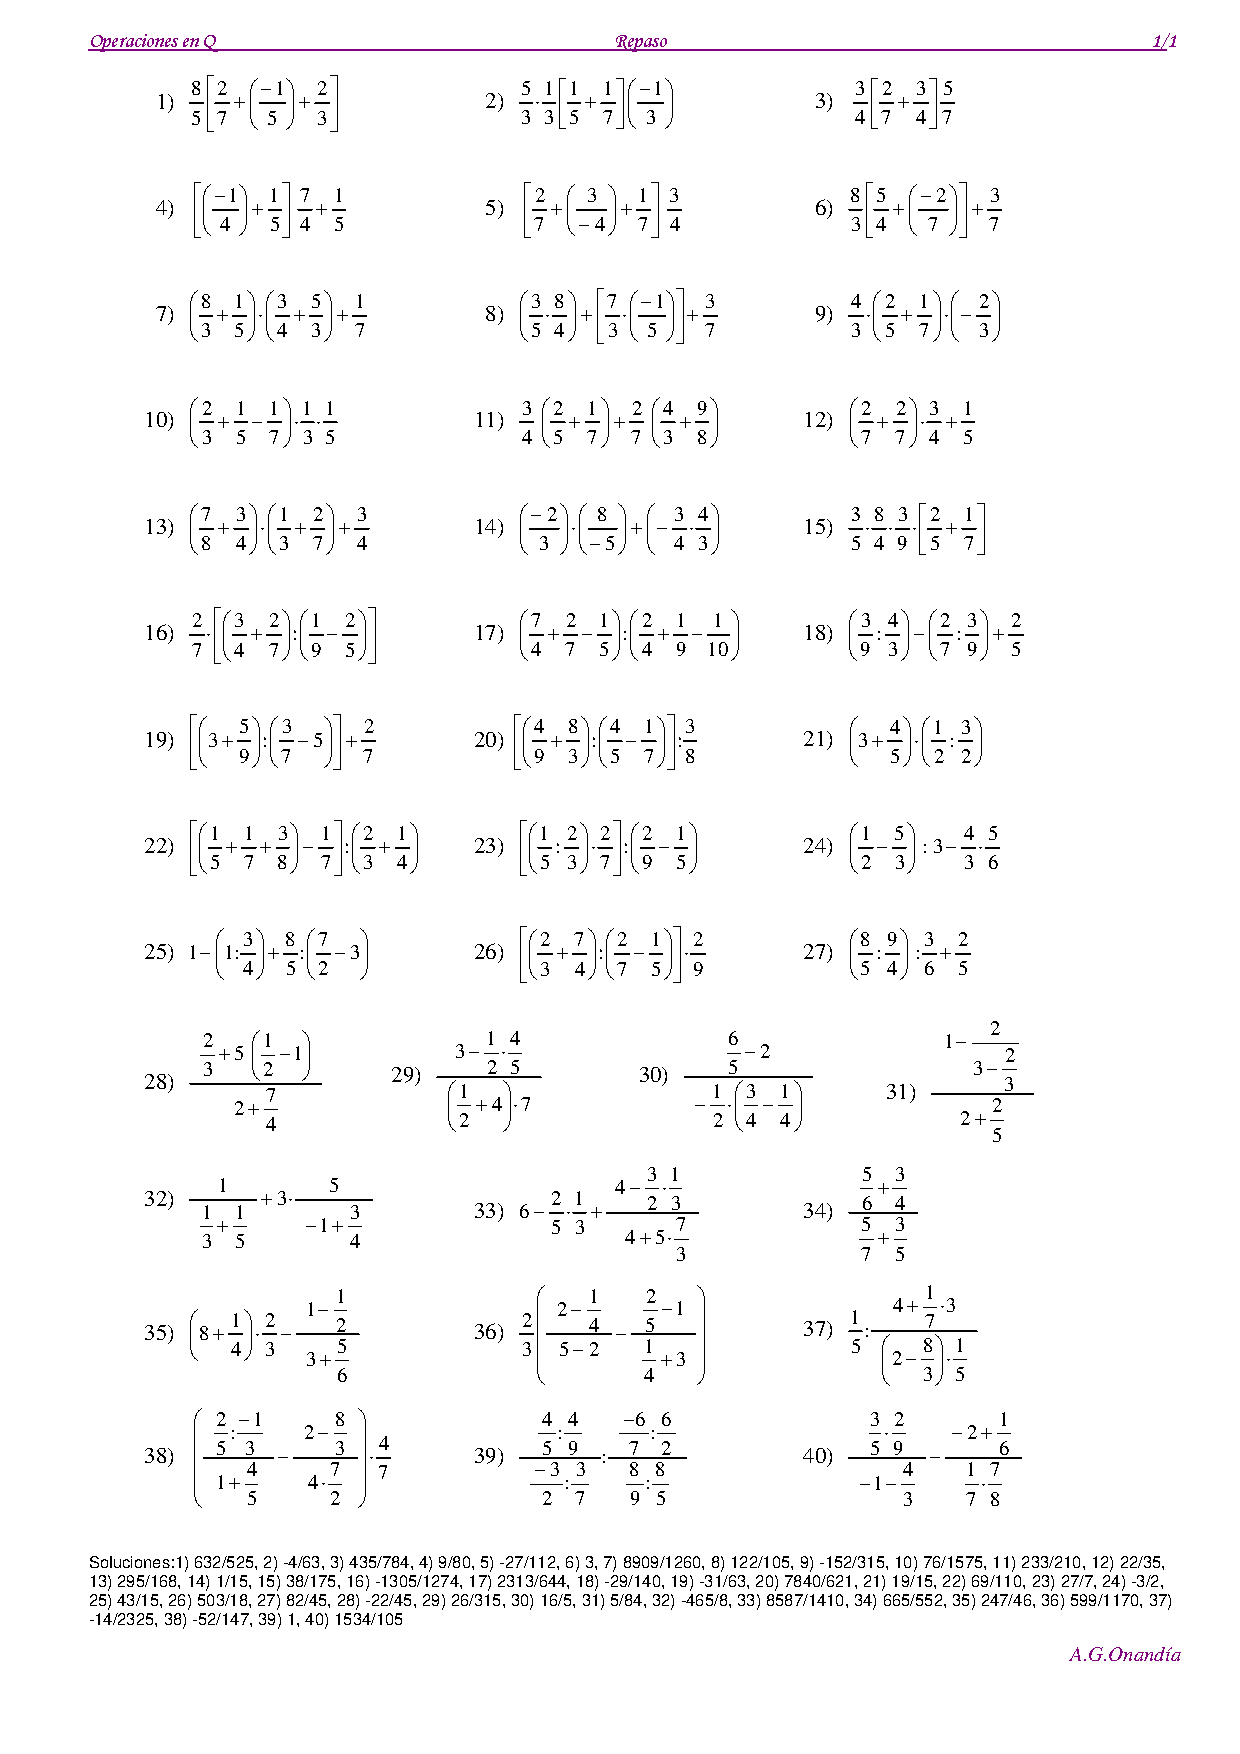
\includepdf[fitpaper=true]{C:/Users/Pedro/Documents/apuntes-particulares/3º de la ESO/Ejercicios/Openq.pdf}
\section{Fracciones como operadores} 

\end{document}